\chapter{Psalm 67}

\begin{figure}
  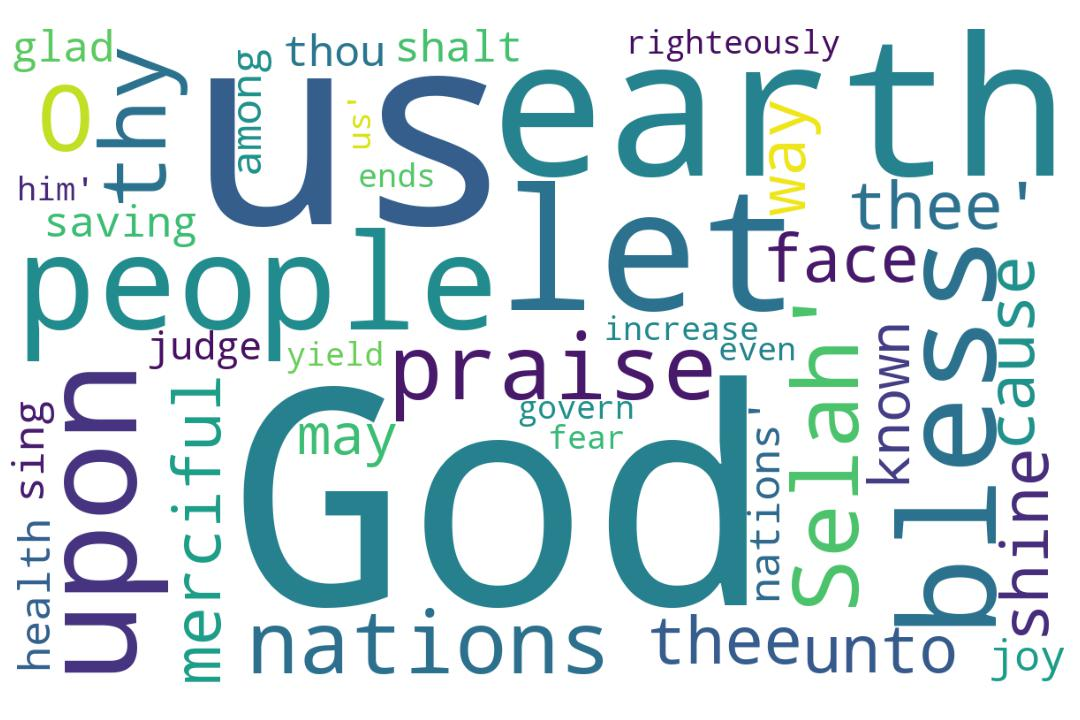
\includegraphics[width=\linewidth]{19OT-Psalms/Psalm67-WordCloud.jpg}
  \caption{Psalm 67 Word Cloud}
  \label{fig:Psalm 67 word Cloud}
\end{figure}


\marginpar{\scriptsize \centering \fcolorbox{bone}{lime}{\textbf{A PLEA FOR MERCY}}\\ (Psalm 67:1-7) \begin{compactenum}[I.][8]
    \item The \textbf{Cause of Comfort} \index[scripture]{Psalms!Psa 067:01}(Psa 67:1)
    \item A \textbf{Corporate Concern} \index[scripture]{Psalms!Psa 067:02}(Psa 67:2)
    \item A \textbf{Common Chorus} \index[scripture]{Psalms!Psa 067:04}(Psa 67:4)
    \item A \textbf{Cure for the Curse} \index[scripture]{Psalms!Psa 067:06}(Psa 67:6)
    \item A \textbf{Comforting Conclusion} \index[scripture]{Psalms!Psa 067:07}(Psa 67:7)
\end{compactenum}}

\footnote{\textcolor[rgb]{0.00,0.25,0.00}{\hyperlink{TOC}{Return to end of Table of Contents.}}}\footnote{\href{https://audiobible.com/bible/psalms_67.html}{\textcolor[cmyk]{0.99998,1,0,0}{Psalm 67 Audio}}}\textcolor[cmyk]{0.99998,1,0,0}{To the chief Musician on Neginoth, A Psalm \emph{or} Song.}\\
\\
\P  \textcolor[cmyk]{0.99998,1,0,0}{God be merciful unto us, and bless us; \emph{and} cause \fcolorbox{bone}{lime}{his face to shine} upon us; Selah.}\footnote{\textbf{Numbers 6:22-27} - And the LORD spake unto Moses, saying, [23] Speak unto Aaron and unto his sons, saying, On this wise ye shall bless the children of Israel, saying unto them, [24] The LORD bless thee, and keep thee: [25] The LORD make his face shine upon thee, and be gracious unto thee: [26] The LORD lift up his countenance upon thee, and give thee peace. [27] And they shall put my name upon the children of Israel; and I will bless them.}%\footnote{The key word to orient the reader shows up twice in seven verses (``Selah'' in verses 1 and 4). By now you know what the ``majority of conservative scholars'' are going to do with it. The entire Psalm deals with the Millennium and the Millennial Reign of the Son of God (see Psalm 2, 110; Isaiah 2, 11, etc.). ``God be merciful unto us and bless us...upon us.'' Verse 1 is a prayer for the restoration of Israel. Note especially the mid-Tribulation (or end-Tribulation) appearance of the Lord from heaven, as in the case of Job (Job 38:1), Saul (Acts 9:4--7), Daniel (Daniel 10:5--11), and Ezekiel (Ezekiel 1:1--4). We have commented on this under Psalm 31:16, which Kroll, Motyer, Yates, Jamieson, Baethgen, Briggs, Ewald, Dummelow, and Hengstenberg went by like they were in the Indianapolis 500. ``Thy saving health'' (vs. 2) is literal (see Psalm 91:3) and extends into eternity for the ``nations'' (see Revelation 22:2). ``All the people praise'' Him (see Psalm 2 and 110), and the ``nations'' will be glad and sing for joy, for the ``fulness of Israel'' (Romans 11:12) will affect nature (see Romans 8:20--27; Isaiah 11:1--10; Amos 9:13, etc.). The characteristics of the Millennium are Joy (vs. 4), Gladness (vs. 4), Blessing (vss. 1--7), Singing (vs. 4), Mercy (vs. 1), Praise (vs. 3), Righteousness (vs. 4), and Increase (vs. 6). This is the “Golden Age” of the unsaved philosophers; the “Thousand Year Reich” of the Nazis; the “Camelot” of the depraved Kennedy family; the “Great Society” of Lyndon Johnson, and the infamous “bringing in of Thy Kingdom” the Southern Baptists wasted their time on. It is the “Our Father” of the pagan Catholics answered at last—“thy kingdom come”— after those depraved killers had been praying it for sixteen hundred years. It came about without their help and despite their efforts, and when it came it destroyed their church, their theology, their priests and nuns, bishops and cardinals, archbishops and popes in one lick, because it was a Jewish kingdom (Luke 1:32). “Salvation is of the Jews” (John 4:22). Rome was never given the privilege, at either Advent, of saving anyone. \cite{Ruckman1992Psalms} }
[2] \textcolor[cmyk]{0.99998,1,0,0}{That thy way may be known upon earth, thy saving health \fcolorbox{bone}{lime}{among all nations}.} %\footnote{Ready for chaos? Here it is: ``May the people praise you...for you rule [present tense] the people justly'' (verses 3--4). This is the aborted perversion known as the New International Version. It simply erased the Millennial references. The nation’s knowledge of God is not even conditioned on God blessing Israel in the NIV, for the words “That thy way may be known” (vs. 2) have been removed from it. This is the godless abomination that bragged about how much more “readable” it was than the King James Bible and proved it by testing it out with a couple of hundred dead orthodox apostate kiddy school readers attached to dead orthodox churches. Not even the RSV of the NCC was this corrupt, although The Living Bible was; it did the same thing in order to disconnect the knowledge of God by the nations with the coming of the Lord. The Living Bible even destroys the sense of verse 1 by making it a present tense: ``as you look down on us.'' Kyle Yates (RSV committee) tells us that the Psalm is “Remarkable for its beauty, its simplicity and its world outlook.” (Can’t you guess what he is going to do? You get one guess!) “God’s gracious dealings are viewed as the means by which all people are led to turn to God...this is a striking universalistic note...expressing hope for God’s continued blessing in order that Israel’s mission may be completed.” \cite{Ruckman1992Psalms}} 
[3] \textcolor[cmyk]{0.99998,1,0,0}{Let the people praise thee, O God; let all the people praise thee.}
[4] \textcolor[cmyk]{0.99998,1,0,0}{O let the nations be glad and \fcolorbox{bone}{lime}{sing for joy}: for thou shalt judge the people righteously, and govern the nations upon earth. Selah.} %\footnote{Interpretation? “Rapunzel, Rapunzel, let down your golden hair.” No Advent, no return of Christ, no throne at Jerusalem, no Jesus Christ, no scriptural fulfillment, no restoration of Israel: just one big, godless, hellish, damnable denial of the main theme of the Bible, laden with enough piety and “godliness” to “gag a maggot” (circa 1980, Middle Schools). Kroll, being Premillennial, is finally forced to show his hand at verse 4, but not till then. He disassociates verse 1 from the Tribulation and the Advent and does away with the “saving health” by saying contemptuously it is “to be understood in the singular sense as salvation among all nations.” He didn’t make any connection with “health” at all, as it was given in Psalm 91:3; Ezekiel chapter 47; and Revelation 22:2; he equated “health” with Church Age salvation. Poor old Dummelow splashes around like a crippled thrasher in a bird bath. He wants the RV reading of Westcott and Hort put back into verses 4 and 6 and says that “God’s goodness to Israel reveals him [present tense] to the nations,” which of course is more nonsense. But Jamieson and Brown have the best way of saying what you don’t mean so you will think they mean what they think they didn’t say: “The manifest blessedness of Israel IN HER LORD shall attract all nations to the same Saviour...when all the people praise God then the earth itself shall be delivered from the curse...the future is to the eye of inspiration as sure as the already past...God’s blessing on the literal and spiritual Israel shall be the FORERUNNER of the conversion of the world.” Beautiful, ain’t it? No date given, no Lord returning, no Lord landing, no Lord reigning, no judgment on the nations, no judging the nations literally on earth, and no renovation of nature because of the King’s presence. The “blessing” came from people praising God. Dale Carnegie, Chuck Swindoll, Robert Schuller, and Norman Vincent Peale never did it any better. This is a typical masterpiece of “toning down,” “leavening,” and “stripping” a passage of its Biblical content. It is a dehydrating, blood letting, artificial preservative type of exposition that fills the works of the “godly scholars.” In the raw it is simply two things: unbelief and cowardice. \cite{Ruckman1992Psalms} }
[5] \textcolor[cmyk]{0.99998,1,0,0}{Let the people praise thee, O God; let all the people praise thee.}
[6] \textcolor[cmyk]{0.99998,1,0,0}{\emph{Then} shall the earth yield her increase; \emph{and} God, \emph{even} our own God, \fcolorbox{bone}{lime}{shall bless us}.}
[7] \textcolor[cmyk]{0.99998,1,0,0}{God shall bless us; and all the \fcolorbox{bone}{lime}{ends of the earth} shall fear him.}